\documentclass[a4paper,12pt,bibliography=totocnumbered]{scrartcl}

\usepackage[utf8]{inputenc} 
\usepackage[T1]{fontenc}
\usepackage[ngerman]{babel} 
\usepackage{amsmath, amssymb,amsfonts}
\usepackage{graphicx}
\usepackage{csquotes}
\usepackage[bookmarks,colorlinks=true]{hyperref}
\usepackage{geometry}
\usepackage{float}
\usepackage[final]{pdfpages}
\usepackage{framed, color} 
\usepackage{scrlayer-scrpage}
\usepackage{siunitx}
\usepackage{subfigure}
\renewcaptionname{ngerman}{\figurename}{Abb.}
\sisetup{detect-weight=true, detect-family=true,locale=DE,range-phrase={\,bis\,},list-final-separator ={\,\linebreak[0] \text{und}\,},separate-uncertainty=true,per-mode = symbol-or-fraction}
\DeclareSIUnit\curie{Ci}
\usepackage[backend=biber, style=chem-angew]{biblatex} 
\addbibresource{lit.bib} 

\usepackage{chemgreek}
\usepackage{chemformula}

\urlstyle{same}
%Hyperlinks-Setup
\hypersetup{
	colorlinks,
	linktocpage,
	citecolor=black,
	filecolor=black,
	linkcolor=black,
	urlcolor=black
}

%\numberwithin{equation}{section}

\setlength{\parindent}{0 mm}
\setlength{\parskip}{2 mm} 



\pagestyle{scrheadings}
%Header oben links auf linker Seite (ungerade Seitenzahl) und oben rechts auf rechter Seite (gerade Seitenzahl), beinhaltet gruppennummer und Versuchskürzel. Im Fall eine einseitigen Dokuments: Header oben rechts
\ihead{\VerfasserEINS\;\&\;\VerfasserZWEI} %Header oben rechts auf linker Seite und oben links auf rechter Seite. Beinhaltet die Namen der Verfasser. Im Fall eine einseitigen Dokuments: Header oben links!
\ofoot{\thepage} %Footer unten links auf linker und unten rechts auf rechter Seite, enthält die jeweilige Seitenzahl. Im Fall eines einseitigen Elements: Footer unten rechts!
\cfoot{\empty} %Mittig unten im Footer soll nichts eingetragen werden 
\ifoot{\empty} %Footer unten rechts auf linker und unten links auf rechter Seite. Hier ebenfalls leer.


\newcommand{\VERSUCHSDATUM}{20.10.-27.10.2025}
\newcommand{\PROTOKOLLDATUM}{\today}

\newcommand{\VerfasserEINS}{Vincent Kümmerle}
\newcommand{\MatNoEINS}{3712667}
\newcommand{\EmailEINS}{st187541@stud.uni-stuttgart.de}
\newcommand{\StudiengangEINS}{B.Sc. Chemie}

\newcommand{\VerfasserZWEI}{Elvis Gnaglo}
\newcommand{\MatNoZWEI}{3710504}
\newcommand{\EmailZWEI}{st189318@stud.uni-stuttgart.de}
\newcommand{\StudiengangZWEI}{B.Sc. Chemie}

\newcommand{\BETREUER}{Benjamin Knies}
\newcommand{\GRUPPENNR}{A05}

\newcommand{\VERSUCHSNR}{Festkörper Präparat}
\newcommand{\VERSUCHSNAME}{Cobalteisenstein}


\begin{document}
\thispagestyle{empty}


\begin{titlepage}

\begin{center}
\Huge{\textbf{\VERSUCHSNR\ - \VERSUCHSNAME}}\\
\vspace{10mm}% Abstand
\Large{Protokoll zum Versuch des AC2 Praktikums von \\ \textbf{\VerfasserEINS\;\& \VerfasserZWEI}}\\
\vspace{10mm} 
\Large{Universität Stuttgart}\\
\end{center}
\vspace{1cm}
\begin{center}
\begin{tabular}{ll}
\large{Verfasser:}		& \large{\VerfasserEINS,} \large{\MatNoEINS} \\
 						& \large{\EmailEINS} \\
 						\vspace{0cm}\\
						& \large{\VerfasserZWEI,} \large{\MatNoZWEI} \\
                        & \large{\EmailZWEI} \\
						\vspace{0cm}\\
\large{Gruppennummer:}	& \large{\GRUPPENNR} \\
\vspace{0cm}\\
\large{Versuchszeitraum:}	& \large{\VERSUCHSDATUM} \\
\vspace{0cm}\\
\large{Betreuer:}		& \large{\BETREUER} \\
\vspace{0cm}\\
\large{Abgabenummer:} & \large{1. Abgabe}
\end{tabular}
\end{center}
\vspace{15mm}

\begin{center}
Stuttgart, den \PROTOKOLLDATUM
\end{center}

\end{titlepage}


\thispagestyle{empty}

\tableofcontents 

\clearpage

\renewcommand{\thepage}{\arabic{page}}
\setcounter{page}{1}


\section{Einleitung}
In der Vergangenheit weckte Cobalteisenstein durch Untersuchung des hohen elektrischen Widerstands, der hohen Remanenz und Koerzitivkraft in den frühen 1930er Jahren in Japan erstmals Interesse, bevor es als nichtleitender Permanentmagnet ab Anfang 1950 durch das günstiger herzustellende Bariumferrit abgelöst wurde.
\cite{History}.
Heutzutage finden Cobaltferritnanopartikel Verwendung für Magnetspeichersysteme mit hoher Kapazität und \ch{CoFe2O4} wird zudem als Katalysator für die Oxidation von Alkenen genutzt. \cite{Rieck}
Cobalteisenstein kristallisiert in der Spinellstruktur und weist die Raumgruppe $Fd \overline{3} m$ auf. 
Im Zuge der Strukturbeschreibung stellt sich die Frage nach der Kationenverteilung. 
Dazu wird die Ligandenfeldaufspaltungsstabilisierungsenergie (LSFE) im inversen Spinell mit \ch{Co^{2+}} in den Oktaederlücken im Vergleich zum normalen Spinell mit \ch{Co^{2+}} in den Tetraederlücken berechnet. 
Da die LSFE im inversen Spinell höher ist, ergibt sich für den inversen Spinell eine günstigere Stabilisierung.
Die in \autoref{fig: Elementarzelle} dargestellte Elementarzelle des Cobalteisensteins besteht aus einer kubisch-dichtesten Kugelpackung der \ch{O^{2-}}-Anionen, wobei $\frac{1}{8}$ der Tetraederlücken mit \ch{Fe^{3+}}, 
$\frac{1}{4}$ der Oktaederlücken mit \ch{Fe^{3+}} und $\frac{1}{4}$ der Oktaederlücken mit \ch{Co^{2+}} besetzt sind. \\

\begin{figure}[H]
    \centering
    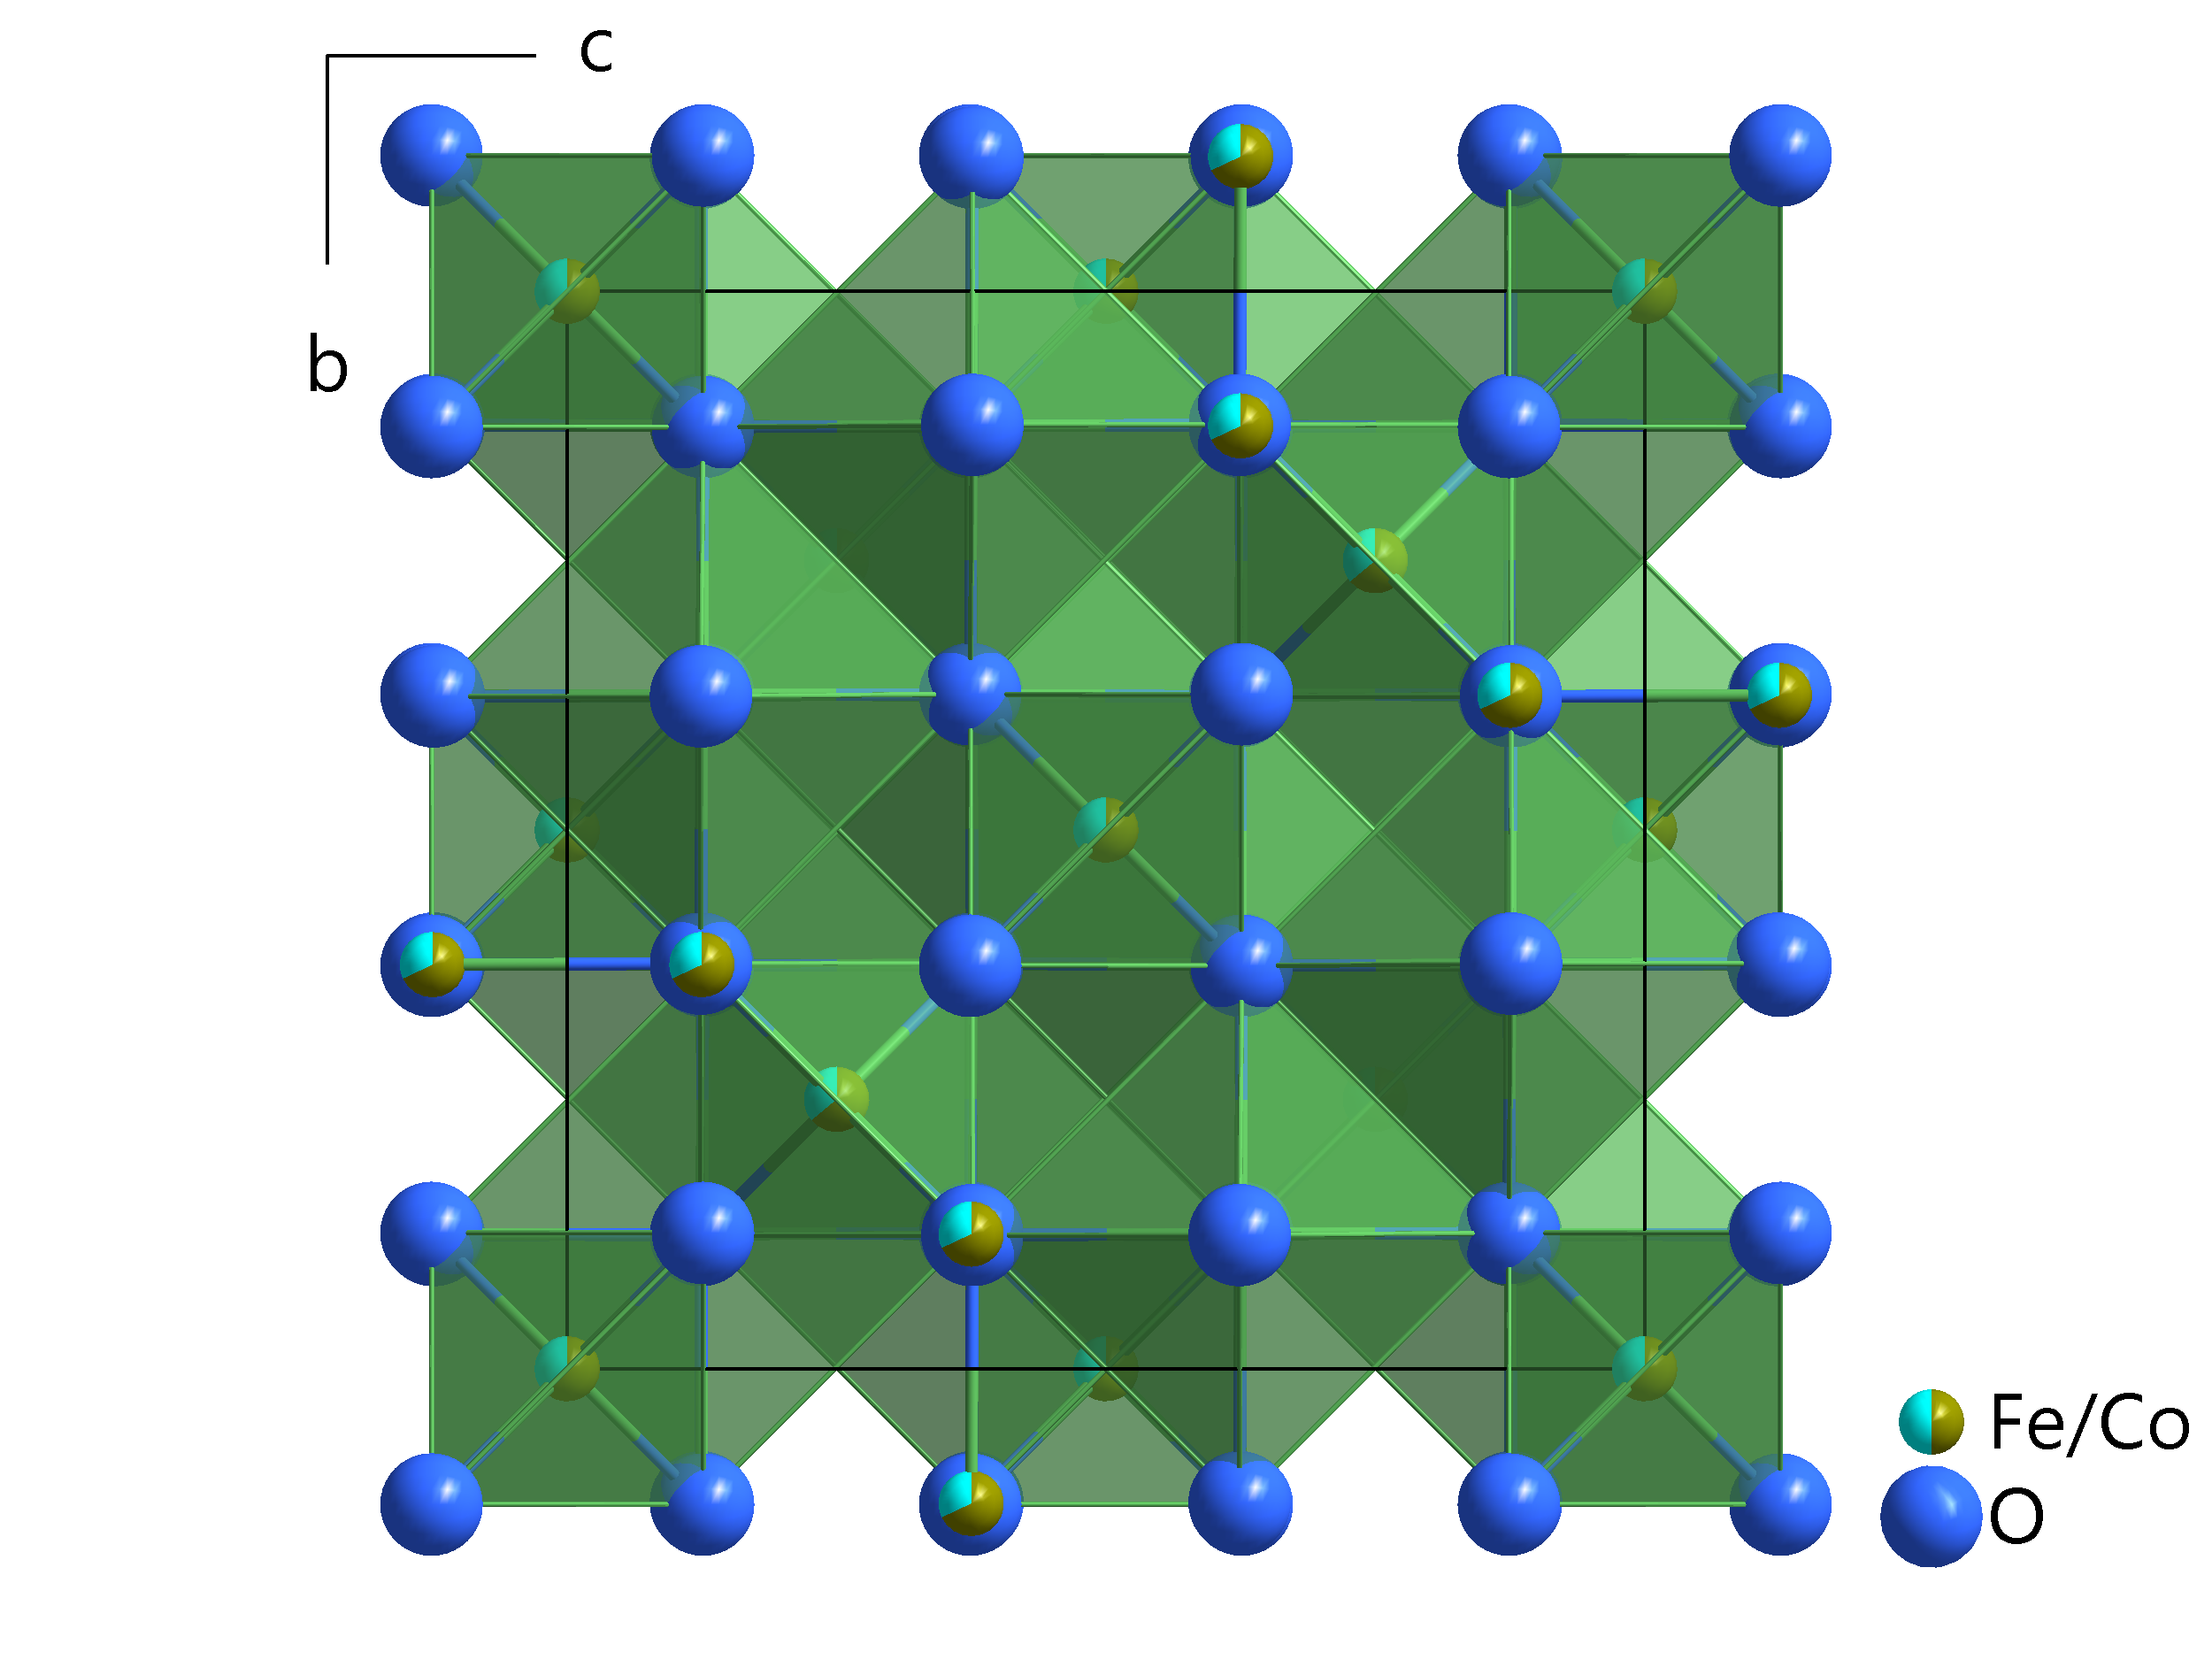
\includegraphics[scale=0.2]{Elementarzelle.png}
    \caption{Elementarzelle des \ch{CoFe2O4}.\cite{Rieck}}
    \label{fig: Elementarzelle}
\end{figure}

Tatsächlich sind die Kationen jedoch zufällig auf die Tetraeder- und Oktaederlücken verteilt \cite{Rieck}.
Dies lässt sich darauf zurückführen, dass \ch{Co^{2+}} einen kleineren Ionenradius als \ch{Fe^{3+}} aufweist und somit auch die Tetraederlücken besetzt, da diese eine geringe Bindungslänge zwischen Zentralkation und den \ch{O^{2-}}-Anionen als die Oktaederlücken aufweist.
Dies ist im Strukturausschnitt in \autoref{fig: TL} aufgezeigt, in dem vier Anionen tetraedrisch um ein Metallkation angeordnet sind, wohingegen es in der Oktaederlücke in \autoref{fig: OL} sechs Anionen sind.


\begin{figure}[H]
    \centering
    \includegraphics[scale=0.1]{Tetraederlücke.png}
    \caption{Tetraederlücken in \ch{CoFe2O4}.\cite{Rieck}}
    \label{fig: TL}
\end{figure}

\begin{figure}[H]
    \centering
    \includegraphics[scale=0.15]{Oktaederlücke.png}
    \caption{Oktaederlücken in \ch{CoFe2O4}.\cite{Rieck}}
    \label{fig: OL}
\end{figure}

\section{Charakterisierungsmethoden}
Die hergestellte Verbindung wird mit Hilfe der Pulverdiffraktometrie charakterisiert.
Dabei werden Elektronen über eine Heizspannung aus einer Wolframkathode in das Vakuum der Röntgenröhre geleitet und über die dort angelegte Spannung zur Kupferanode beschleunigt. 
An der Anode können die freien Elektronen auf Elektronen in den inneren Schalen treffen und diese "herausschlagen".
%Bild RÖhre
Der dadurch erzeugte Elektronenmangel in der Schale wird durch ein Elektron aus einer höheren Schale ausgeglichen, wobei dieses beim Wechseln der Schalen Energie in Form von charakteristischer Röntgenstrahlung freisetzt. 
Einige Elektronen dringen stattdessen bis zum Atomkern vor. 
Dort werden sie durch Wechselwirkungen mit dem Kern unter Abgabe von Röntgenstrahlung als Bremsstrahlung mit vielen verschiedenen Wellenlängen abgelenkt.
Daher wird die austretende Strahlung über einen Polarisator gefiltert, bevor sie auf die Probe trifft. 
Durch Ablenkung der Röntgenstrahlung am Kristallgitter der Probe, können Beugungsreflexe detektiert werden, die durch ihre Intensität und räumliche Anordnung auf die Geometrie des Kristallgitters schließen lassen.

\newpage

\section{Durchführung}
\ch{Co3O4}(85 mg; 0,352 mmol) und \ch{Fe2O3}(170 mg; 1,066 mmol) wurden abgewogen und im Mörser zu einem feinen Pulver zerkleinert. 
Anschließend wurde das Gemisch in einen Porzellantiegel überführt und für 48 Stunden bei $800 ^\circ$C im Ofen erhitzt.\\
Nach Abkühlen an der Luft wurde ein dunkelgraues Pulver erhalten. 
Dieses wurde anschließend erneut mit dem Mörser zu einem feinen Pulver gemahlen und auf den Probenträger des Pulverdiffraktometers getragen. 
Der Probenträger wurde danach in das Pulverdiffraktometer gespannt und die Probe wurde für 20 Minuten unter Drehung analysiert.

\section{Ergebnisse}




\cite{FeDiff}

\section{Zusammenfassung}



\printbibliography[title={Literatur}]


\end{document}
